% Figure 1 -- VCF-RDFizer v3.1.0 pipeline.
% Standalone TikZ source; build with: pdflatex vcf2rdf-v3.tex  ->  vcf2rdf-v3.pdf
% Drawn at the journal text width (372pt, about 13.1 cm) so it is included unscaled.
\documentclass[border=2pt]{standalone}
\usepackage[T1]{fontenc}
\usepackage{helvet}
\renewcommand{\familydefault}{\sfdefault}
\usepackage{tikz}
\usetikzlibrary{arrows.meta,positioning,fit,calc,backgrounds,shapes.geometric}

\definecolor{cvcf}{HTML}{F6E3B4}   \definecolor{cvcfd}{HTML}{C9A227}
\definecolor{ctsv}{HTML}{FBE3E3}   \definecolor{ctsvd}{HTML}{C00000}
\definecolor{crml}{HTML}{B7E3E4}   \definecolor{crmld}{HTML}{1F7F83}
\definecolor{cnt}{HTML}{EEEEEE}    \definecolor{cntd}{HTML}{555555}
\definecolor{chdt}{HTML}{E5D9F0}   \definecolor{chdtd}{HTML}{7030A0}
\definecolor{ccot}{HTML}{FCE4CC}   \definecolor{ccotd}{HTML}{C55A11}
\definecolor{cval}{HTML}{DDEFD9}   \definecolor{cvald}{HTML}{2E7D32}
\definecolor{cpkg}{HTML}{DCE6F5}   \definecolor{cpkgd}{HTML}{2F5597}
\definecolor{cband}{HTML}{F7F7F7}

\begin{document}
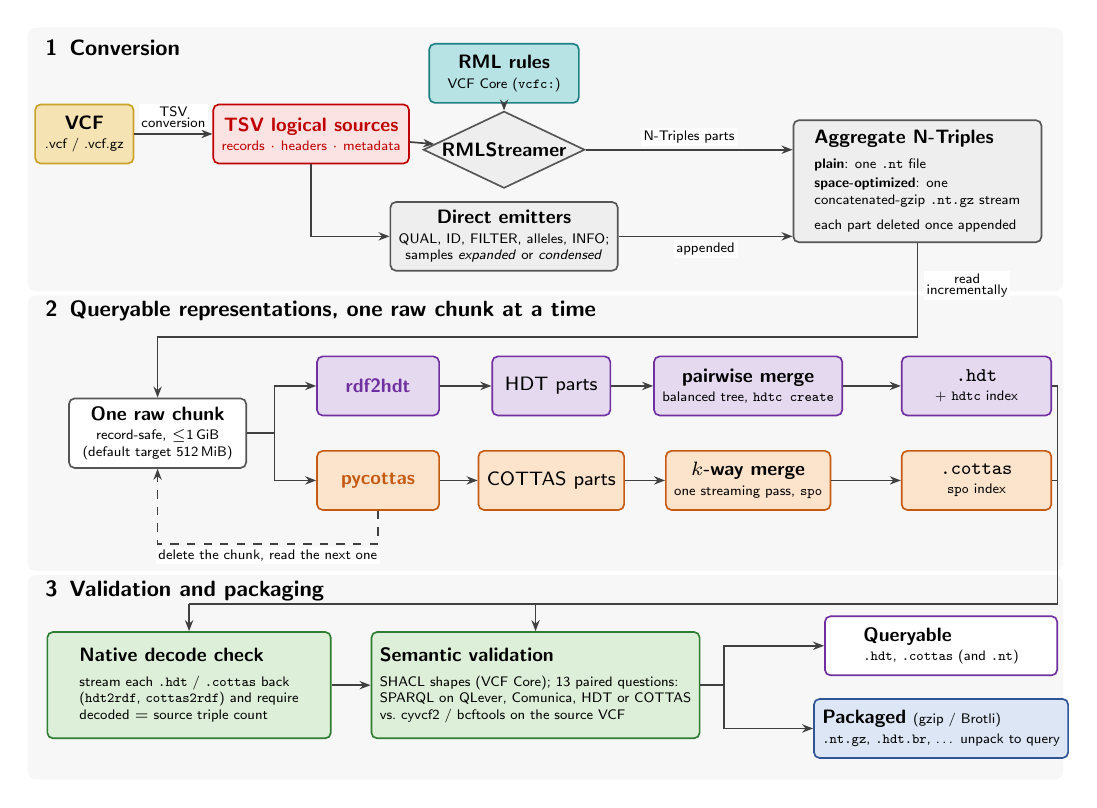
\begin{tikzpicture}[
  font=\scriptsize,
  >={Stealth[length=4pt]},
  box/.style={draw, rounded corners=2pt, line width=0.6pt, align=center, inner sep=3pt, minimum height=0.75cm},
  flow/.style={->, line width=0.6pt, draw=black!75},
  dflow/.style={->, line width=0.6pt, draw=black!75, dashed},
  lbl/.style={font=\tiny, fill=white, inner sep=1pt, align=center},
  band/.style={font=\footnotesize\bfseries\itshape, anchor=west},
]

% ------------------------------------------------------------------ band 1
\node[band] at (0,0.35) {1\enspace Conversion};

\node[box, fill=cvcf, draw=cvcfd, minimum width=1.25cm] (vcf) at (0.62,-0.75) {\textbf{VCF}\\[-1pt]\tiny .vcf / .vcf.gz};

\node[box, fill=ctsv, draw=ctsvd, text=ctsvd, minimum width=2.1cm] (tsv) at (3.5,-0.75)
  {\textbf{TSV logical sources}\\[-1pt]\tiny records $\cdot$ headers $\cdot$ metadata};

\node[box, fill=crml, draw=crmld, minimum width=1.9cm] (rml) at (5.95,0.02)
  {\textbf{RML rules}\\[-1pt]\tiny VCF Core (\texttt{vcfc:})};

\node[diamond, aspect=2.1, draw=cntd, fill=cnt, line width=0.6pt, inner sep=0.5pt, font=\scriptsize\bfseries] (rmls) at (5.95,-0.95) {RMLStreamer};

\node[box, fill=cnt, draw=cntd, minimum width=2.6cm] (emit) at (5.95,-2.05)
  {\textbf{Direct emitters}\\[-1pt]\tiny QUAL, ID, FILTER, alleles, INFO;\\[-2pt]\tiny samples \emph{expanded} or \emph{condensed}};

\node[box, fill=cnt, draw=cntd, minimum width=3.15cm, minimum height=1.55cm, align=left] (agg) at (11.2,-1.35)
  {\textbf{Aggregate N-Triples}\\[1pt]
   \tiny \textbf{plain}: one \texttt{.nt} file\\[-1pt]
   \tiny \textbf{space-optimized}: one\\[-2pt]
   \tiny concatenated-gzip \texttt{.nt.gz} stream\\[1pt]
   \tiny each part deleted once appended};

\draw[flow] (vcf) -- node[lbl, above=1pt]{TSV\\[-2pt]conversion} (tsv);
\draw[flow] (tsv) -- (rmls);
\draw[flow] (rml) -- (rmls);
\draw[flow] (tsv.south) |- (emit.west);
\draw[flow] (rmls.east) -- node[lbl, above=1pt]{N-Triples parts} (rmls.east -| agg.west);
\draw[flow] (emit.east) -- node[lbl, below=1pt]{appended} (emit.east -| agg.west);

% ------------------------------------------------------------------ band 2
\node[band] at (0,-3.0) {2\enspace Queryable representations, one raw chunk at a time};

\node[box, fill=white, draw=cntd, minimum width=2.25cm] (chunk) at (1.55,-4.55)
  {\textbf{One raw chunk}\\[-1pt]\tiny record-safe, $\leq$1\,GiB\\[-2pt]\tiny (default target 512\,MiB)};

\draw[flow] (agg.south) -- node[lbl, pos=0.45, right=2pt]{read\\[-2pt]incrementally} (agg.south |- 0,-3.33) -- (chunk.north |- 0,-3.33) -- (chunk.north);

\node[box, fill=chdt, draw=chdtd, text=chdtd, minimum width=1.55cm] (r2h) at (4.35,-3.95) {\textbf{rdf2hdt}};
\node[box, fill=ccot, draw=ccotd, text=ccotd, minimum width=1.55cm] (r2c) at (4.35,-5.15) {\textbf{pycottas}};

\draw[flow] (chunk.east) -- ++(0.35,0) |- (r2h.west);
\draw[flow] (chunk.east) -- ++(0.35,0) |- (r2c.west);

\node[box, fill=chdt, draw=chdtd, minimum width=1.5cm] (hparts) at (6.55,-3.95) {HDT parts};
\node[box, fill=ccot, draw=ccotd, minimum width=1.5cm] (cparts) at (6.55,-5.15) {COTTAS parts};
\draw[flow] (r2h) -- (hparts);
\draw[flow] (r2c) -- (cparts);

% delete-and-repeat loop: both builders consume the chunk, then it is deleted
\draw[dflow] (r2c.south) -- ++(0,-0.42) -| node[lbl, pos=0.25, below=1pt]{delete the chunk, read the next one} (chunk.south);

\node[box, fill=chdt, draw=chdtd, minimum width=2.05cm] (hmerge) at (9.05,-3.95)
  {\textbf{pairwise merge}\\[-1pt]\tiny balanced tree, \texttt{hdtc create}};
\node[box, fill=ccot, draw=ccotd, minimum width=2.05cm] (cmerge) at (9.05,-5.15)
  {\textbf{$k$-way merge}\\[-1pt]\tiny one streaming pass, \texttt{spo}};
\draw[flow] (hparts) -- (hmerge);
\draw[flow] (cparts) -- (cmerge);

\node[box, fill=chdt, draw=chdtd, minimum width=1.9cm] (hdt) at (11.95,-3.95)
  {\textbf{\texttt{.hdt}}\\[-1pt]\tiny + \texttt{hdtc} index};
\node[box, fill=ccot, draw=ccotd, minimum width=1.9cm] (cot) at (11.95,-5.15)
  {\textbf{\texttt{.cottas}}\\[-1pt]\tiny \texttt{spo} index};
\draw[flow] (hmerge) -- (hdt);
\draw[flow] (cmerge) -- (cot);

% ------------------------------------------------------------------ band 3
\node[band] at (0,-6.55) {3\enspace Validation and packaging};

\node[box, fill=cval, draw=cvald, minimum width=3.6cm, minimum height=1.35cm, align=left] (decode) at (1.95,-7.75)
  {\textbf{Native decode check}\\[1pt]
   \tiny stream each \texttt{.hdt} / \texttt{.cottas} back\\[-2pt]
   \tiny (\texttt{hdt2rdf}, \texttt{cottas2rdf}) and require\\[-2pt]
   \tiny decoded $=$ source triple count};

\node[box, fill=cval, draw=cvald, minimum width=4.1cm, minimum height=1.35cm, align=left] (sem) at (6.35,-7.75)
  {\textbf{Semantic validation}\\[1pt]
   \tiny SHACL shapes (VCF Core); 13 paired questions:\\[-2pt]
   \tiny SPARQL on QLever, Comunica, HDT or COTTAS\\[-2pt]
   \tiny vs.\ cyvcf2 / bcftools on the source VCF};

\node[box, fill=white, draw=chdtd, minimum width=2.95cm, align=left] (qry) at (11.5,-7.25)
  {\textbf{Queryable}\\[-1pt]\tiny \texttt{.hdt}, \texttt{.cottas} (and \texttt{.nt})};
\node[box, fill=cpkg, draw=cpkgd, minimum width=2.95cm, align=left] (pkg) at (11.5,-8.3)
  {\textbf{Packaged} \tiny (gzip / Brotli)\\[-1pt]\tiny \texttt{.nt.gz}, \texttt{.hdt.br}, \dots\ unpack to query};

\draw[line width=0.6pt, draw=black!75] (hdt.east) -- (12.98,-3.95);
\draw[line width=0.6pt, draw=black!75] (cot.east) -- (12.98,-5.15);
\draw[line width=0.6pt, draw=black!75] (12.98,-3.95) -- (12.98,-6.72) -- (decode.north |- 0,-6.72);
\draw[flow] (decode.north |- 0,-6.72) -- (decode.north);
\draw[flow] (sem.north |- 0,-6.72) -- (sem.north);
\draw[flow] (sem.east) -- ++(0.3,0) |- (qry.west);
\draw[flow] (sem.east) -- ++(0.3,0) |- (pkg.west);
\draw[flow] (decode.east) -- (sem.west);

% ------------------------------------------------------------------ band backgrounds
\begin{scope}[on background layer]
  \fill[cband, rounded corners=3pt] (-0.1,0.6) rectangle (13.05,-2.75);
  \fill[cband, rounded corners=3pt] (-0.1,-2.8) rectangle (13.05,-6.3);
  \fill[cband, rounded corners=3pt] (-0.1,-6.35) rectangle (13.05,-8.95);
\end{scope}
\end{tikzpicture}
\end{document}
